\documentclass[a4paper, 12pt]{article}
\usepackage{../../Templates/package}
\usepackage{amssymb}
\usepackage{graphicx}
\usepackage[export]{adjustbox}
\usepackage{framed}
\graphicspath{{../../Assets}}

\newcommand{\Titolo}{Manuale Utente}
\newcommand{\Data}{10/05/2024}
\newcommand{\Versione}{1.0.0}
\newcommand{\Descrizione}{Questo documento fornisce istruzioni dettagliate sull'utilizzo della \textit{web app} EasyMeal.}
\newcommand{\Verificatori}{
    Alessandro Tigani Sava, Matteo Bando, \\
    & Giacomo Gualato, Davide Maffei, \\
    & Niccolò Carlesso, Carlo Rosso     
}
\newcommand{\Redattori}{ 
    Alessandro Tigani Sava, Matteo Bando, \\
    & Giacomo Gualato, Davide Maffei, \\
    & Niccolò Carlesso, Carlo Rosso     
}
\newcommand{\Approvatori}{Giacomo Gualato}
\newcommand{\Destinatari}{
    Prof.\ Tullio Vardanega \\ 
    & Prof.\ Riccardo Cardin \\ 
    & Alessandro Staffolani
}
\newcommand{\Stato}{Approvato}

\newcommand{\Gruppo}{SWEnergy}
\newcommand{\Mail}{\href{mailto:project.swenergy@gmail.com}{project.swenergy@gmail.com}}

\renewcommand\familydefault{\sfdefault} % Set default font family to sans-serif
\linespread{1.5}

\hypersetup{
	pdfmenubar=true,            % show Acrobat’s menu?
	pdfstartview={FitH},        % fits the width of the page to the window
	colorlinks=true,            % false: boxed links; true: colored links
	linkcolor=black,            % color of internal links (change box color with linkbordercolor)
	% citecolor=green,          % color of links to bibliography
	% filecolor=magenta,        % color of file links
	urlcolor=[RGB]{156,1,198}   % color of external links
}

\newcommand{\copertina}{
	\begin{titlepage}
		\vspace*{-3.5cm}
		\makebox[\textwidth]{
\includegraphics[width=\paperwidth]{header.png}}
		\begin{center}
			
\includegraphics[width=1\textwidth]{logo.png}	\\
			\vspace{1cm}
			\Mail	\\
			\vspace{0.5cm}
			\textbf{\begin{LARGE} \Titolo \end{LARGE}}		\\
			\vspace{1cm}
			\textbf{Descrizione:} \Descrizione{}			\\
			\vspace{1cm}
			\begin{tabular}{ll}
				\textbf{Stato}               & \Stato              \\
				\textbf{Data}                & \Data               \\
				\midrule
				\textbf{Redattori}           & \Redattori          \\
				\textbf{Verificatori}        & \Verificatori       \\

				\ifdefined\Approvatori
				\textbf{Approvatori}         & \Approvatori        \\
				\fi

				\ifdefined\ApprovatoriInterni
				\textbf{Approvatori interni} & \ApprovatoriInterni \\
				\fi

				\ifdefined\ApprovatoriEsterni
				\textbf{Approvatori esterni} & \ApprovatoriEsterni \\
				\fi

				\ifdefined\Destinatari
				\textbf{Destinatari}         & \Destinatari        \\
				\fi

				\midrule

				\ifdefined\Versione
				\textbf{Versione}            & \Versione           \\
				\fi
			\end{tabular}
		\end{center}
		\vspace{4cm}
	\end{titlepage}
	\newpage
}

\fancypagestyle{plain}{
	\fancyhf{}
	\rhead{ 
\includegraphics[scale=0.05]{horizontal_logo.png}}
	\lhead{\Titolo \ifdefined\Versione \ \Versione \fi}
	%\lfoot{\Titolo}
	\rfoot{\thepage{} di \pageref{LastPage}}
	\renewcommand{\headrulewidth}{0.2pt}
	\renewcommand{\footrulewidth}{0.2pt}
}
\pagestyle{plain}


\begin{document}
\copertina{}
\section*{Registro delle modifiche}
 {
  \scriptsize
  \begin{tabular}{p{0.10\linewidth}p{0.10\linewidth}p{0.15\linewidth}p{0.15\linewidth}p{0.15\linewidth}p{0.19\linewidth}}
	  \textbf{Versione} & \textbf{Data} & \textbf{Redattore}     & \textbf{Verificatore} & \textbf{Approvatore} & \textbf{Descrizione}                                                                                                                     \\
	  \toprule
	  2.0.1             & 27/02/2024    & Davide Maffei          & Carlo Rosso           & /                    & Correzioni in seguito alla revisione RTB                                                                                                 \\
	  \hline
	  2.0.0             & 27/02/2024    & /                      & /                     & Niccolò Carlesso     & Approvazione finale del documento                                                                                                        \\
	  \hline
	  1.5.0             & 26/02/2024    & Alessandro Tigani Sava & Carlo Rosso           & /                    & Descrizione metriche di qualità                                                                                                          \\
	  \hline
	  1.4.1             & 14/02/2024    & Davide Maffei          & Giacomo Gualato       & /                    & Allineamento delle sezioni dei ruoli                                                                                                     \\
	  \hline
	  1.4.0             & 14/02/2024    & Davide Maffei          & Giacomo Gualato       & /                    & Creazione delle sezioni dei processi primari, di supporto e organizzativi                                                                \\
	  \hline
	  1.3.0             & 8/01/2024     & Carlo Rosso            & Niccolò Carlesso      & /                    & Correzione della sotto-sezione "Aggiornamento delle "Norme di Progetto"" e aggiunte le sotto-sezioni "Revisione del codice" e "Codifica" \\
	  \hline
	  1.2.0             & 31/12/2023    & Carlo Rosso            & Niccolò Carlesso      & /                    & Ristrutturazione del documento per ruolo, piuttosto che per argomento                                                                    \\
	  \hline
	  1.1.0             & 30/10/2023    & Carlo Rosso            & Giacomo Gualato       & /                    & Aggiornamento della sezione dedicata alla documentazione e aggiunta una sezione dedicata agli appunti                                    \\
	  \hline
	  1.0.0             & 30/10/2023    & /                      & /                     & Giacomo Gualato      & Approvazione finale del documento                                                                                                        \\
	  \hline
	  0.2.1             & 29/10/2023    & Alessandro Tigani Sava & Niccolò Carlesso      & /                    & Modifica procedure in sezione Approvazione di un documento                                                                               \\
	  \hline
	  0.2.0             & 24/10/2023    & Matteo Bando           & Niccolò Carlesso      & /                    & Redazione sezioni Versionamento, Verifica di un documento, Approvazione di un documento                                                  \\
	  \hline
	  0.1.0             & 23/10/2023    & Alessandro Tigani Sava & Matteo Bando          & /                    & Redazione sezioni Introduzione, Strumenti, Creazione e modifica di un documento, Ruoli, Registro delle modifiche                         \\
	  \hline
  \end{tabular}
 }

\newpage

\setcounter{tocdepth}{3}
\tableofcontents
\newpage
\section{Introduzione}

Il presente documento, intitolato "Piano di Progetto", descrive e spiegare le
decisioni organizzative adottate dal gruppo SWEnergy per lo sviluppo del
progetto "\textit{Easy Meal}", proposto dall'azienda
\href{https://imolainformatica.it/}{Imola Informatica}. Il "Piano di Progetto" è
suddiviso nelle seguenti sezioni:

\begin{itemize}
	\item \textbf{Analisi dei rischi}: identifica i rischi individuati dal
	      gruppo e le strategie per mitigarli;

	\item \textbf{Modello di sviluppo}: descrive l'organizzazione temporale del
	      team di SWEnergy;

	\item \textbf{Pianificazione}: dettaglia la pianificazione del lavoro del
	      gruppo, incluse le attività, le risorse e i tempi necessari per lo
	      sviluppo del progetto;

	\item \textbf{Preventivo}: presenta il preventivo delle ore di lavoro e il
	      costo totale del progetto;

	\item \textbf{Consuntivo}: riporta le ore di lavoro e il costo effettivo del
	      progetto fino al momento della stesura del piano di progetto della
	      fase corrente: RTB.
\end{itemize}

\subsection{Scopo del documento}

Questo documento ha lo scopo di raccogliere in modo organico, coerente e
uniforme tutte le informazioni riguardanti la pianificazione del progetto, al
fine di fornire un riferimento per la gestione dello stesso. Al termine della
prima fase del progetto (RTB), verrà utilizzato per valutare l'andamento del
lavoro e per spiegare le decisioni adottate durante la pianificazione.

\subsection{Scopo del prodotto}

"\textit{Easy Meal}" è una web app progettata per gestire le prenotazioni
presso i ristoranti, sia dal lato dei clienti che dei ristoratori. Il prodotto
finale sarà composto da due parti:

\begin{itemize}
	\item \textbf{Cliente}: consente ai clienti di prenotare un tavolo presso un
	      ristorante, visualizzare il menù e effettuare un ordine;

	\item \textbf{Ristoratore}: consente ai ristoratori di gestire le
	      prenotazioni e gli ordini dei clienti, oltre a visualizzare la lista
	      degli ingredienti necessari per preparare i piatti ordinati.
\end{itemize}

\subsection{Glossario}

Al fine di evitare ambiguità linguistiche e garantire un'utilizzazione coerente
delle terminologie nei documenti, il gruppo ha redatto un documento interno
chiamato "Glossario". Questo documento definisce in modo chiaro e preciso i
termini che potrebbero generare ambiguità o incomprensione nel testo. I termini
presenti nel Glossario sono identificati da una 'G' (per esempio parola$_G$) a
pedice.

\subsection{Riferimenti}

\subsubsection{Normativi}
\begin{itemize}
	\item "\textit{Way of Working}";
	\item 	\href{https://www.math.unipd.it/~tullio/IS-1/2023/Progetto/C3.pdf}
	      {Documento del capitolato d'appalto C3 - \textit{Easy Meal}};
	\item \href{https://www.math.unipd.it/~tullio/IS-1/2023/Dispense/PD2.pdf}
	      {Regolamento del progetto};
\end{itemize}

\subsubsection{Informativi}

Slide dell'insegnamento di Ingegneria del Software:
\begin{itemize}
	\item \href{https://www.math.unipd.it/~tullio/IS-1/2023/Dispense/T3.pdf}
	      {Modelli di sviluppo del software};
	\item \href{https://www.math.unipd.it/~tullio/IS-1/2023/Dispense/T4.pdf}
	      {Gestione di progetto};
	\item \href{https://www.math.unipd.it/~tullio/IS-1/2023/Dispense/T5.pdf}
	      {Analisi dei requisiti};
\end{itemize}

\subsection{Scadenze}
Il \textit{team} di SWEnergy si impegna a rispettare le seguenti scadenze per il
completamento del progetto:
\begin{itemize}
	\item \textbf{Prima revisione (avanzamento RTB}: 21 dicembre 2023;
	\item \textbf{Seconda revisione (avanzamento PB)}: da definire;
	\item \textbf{Terza revisione (avanzamento CA)}: da definire;
\end{itemize}

\newpage

\section{Requisiti}
Questa sezione fornisce un elenco dei requisiti minimi indispensabili per l'esecuzione dell'applicazione, illustrando le caratteristiche necessarie per configurare 
correttamente l'ambiente di sviluppo del progetto.

\subsection{Requisiti di sistema}
Affinché l'installazione e l'avvio del prodotto avvengano senza problemi e per garantire un'esperienza completa e soddisfacente nell'utilizzo 
dell'applicazione, è essenziale installare i seguenti \textit{software}.

\begin{longtable}{|c|c|c|}
	\hline
	\textbf{Componente}       & \textbf{ Versione}   & \textbf{ Riferimenti per il download} \\
	\hline
     Node.js             & $ \geq  20.x.x$            &\href{https://nodejs.org/en/}{https://nodejs.org/en/}        \\
    \hline
     npm                & $ \geq 9.x.x$            &Integrato con il download di Node.js        \\
    \hline

    \caption{Tabella dei requisiti di sistema.}
\end{longtable}


\subsection{Requisiti \textit{software}}
L'applicazione è stata testata e confermata come utilizzabile sui principali \textit{browser}, per i quali sono specificate le versioni iniziali che hanno costituito 
il punto di partenza per lo sviluppo del progetto. Durante lo sviluppo, si è considerato incrementalmente l'aggiornamento alle versioni più recenti dei singoli \textit{browser}.

\begin{longtable}{|c|c|c|}
	\hline
	\textbf{Browser}       & \textbf{ Versione}    \\
	\hline
    Google Chrome             & 123                    \\
    \hline
    Arc                       & 1.26                    \\
    \hline
    Opera GX                       & 124                    \\
    \hline
    Safari                        & 17.3                    \\
    \hline
    Microsfot Edge                 & 123                      \\
    \hline

    \caption{Tabella dei requisiti \textit{software}.}
\end{longtable}


\subsection{Requisiti \textit{hardware}}
Poiché l'applicazione funziona su un \textit{browser}, non ci sono requisiti specifici definiti dal proponente, dal capitolato o dal progetto stesso. 
Quindi, i seguenti requisiti sono considerati solo come linee guida generali per l'esecuzione del prodotto creato.

\begin{longtable}{|l|p{0.8\textwidth}|}
	\hline
	\textbf{Componente}       & \textbf{ Requisito minimo}   \\
	\hline
     Processore             &  Processore a 64 bit Quad-Core 3,2 GHz      \\
    \hline
     Memoria RAM            &  4GB DDR4       \\
    \hline
    Spazio su disco         & $ \geq  126 GB$         \\
    \hline
    Connessione Internet         & Connessione \textit{Internet} stabile e veloce, in grado di supportare le esigenze di traffico dell'applicazione         \\
    \hline

    \caption{Tabella dei requisiti \textit{hardware}.}
\end{longtable}
\section{Istruzioni d'uso}

\subsection{Cliente} % --------------------- SECTION DEL CLIENTE ---------------------%

\subsubsection{Accesso cliente}
Questa è la schermata di accesso per il cliente, dove gli utenti non autenticati possono inserire le proprie credenziali di accesso, costituite dall'\textit{email} e dalla {password}. 
Dopo aver compilato i campi, cliccando il pulsante "Accedi", gli utenti verranno reindirizzati alla propria pagina \textit{home} di pertinenza.

\begin{figure}[h]
    \centering
    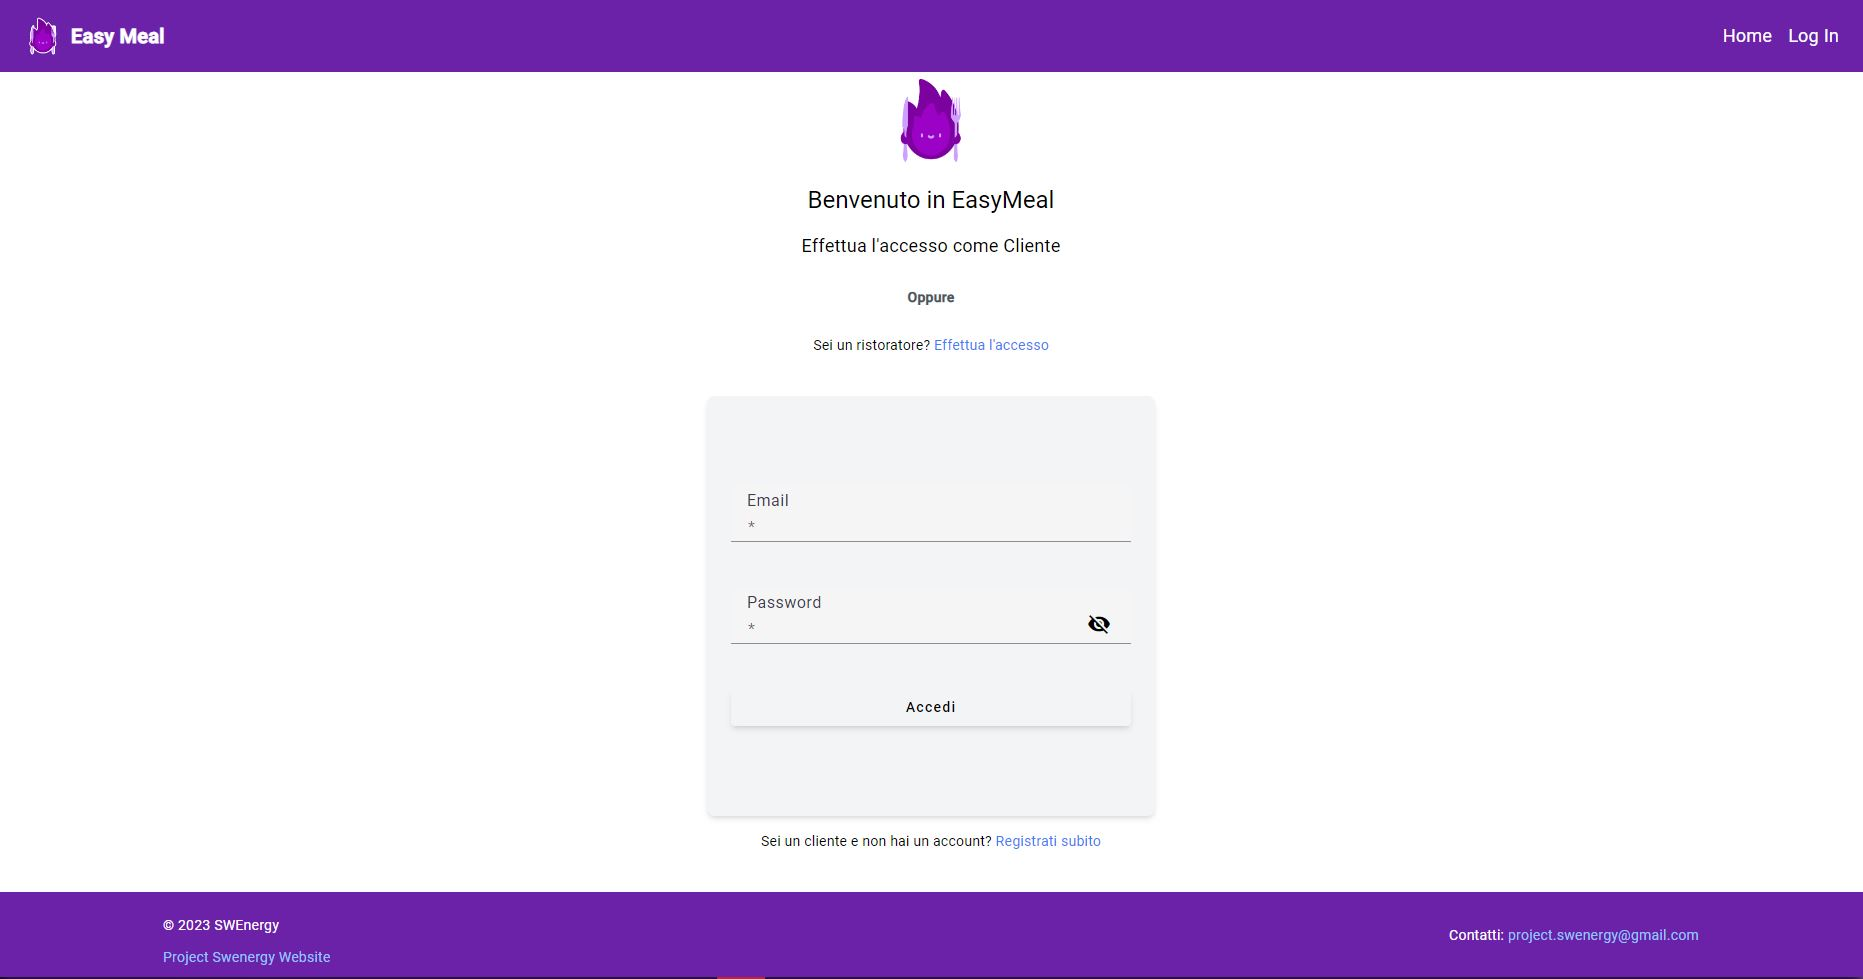
\includegraphics[width=0.9\textwidth]{./img/loginCliente.jpg}
    \caption{Pagina di login del cliente}
    \label{fig:esempio}
\end{figure}

Qui l'utente, nel caso non fosse registrato, può cliccare sul \textit{link} "Registrati subito" per essere reindirizzato alla pagina di registrazione del cliente.
Nel caso l'utente che stia visitando questa pagina non sia un cliente, bensì un ristoratore, può cliccare sul \textit{link} "Sei un ristoratore? Effettua l'accesso" 
per essere reindirizzato alla pagina di accesso del ristoratore.

\subsubsection{Permessi non corretti}
Se l'utente non fosse autenticato ad accedere ad una determina pagina, verrò reindirizzato alla seguente schermata:
IMMAGINE DA INSERIRE

\subsubsection{Pagina inesistente}
SE SI FA NEL MVP ALLORA VA MESSA + IMMAGINE, ALTRIMENTI SI CANCELLA QUELLO SCRITTO:
Si noti che se l'utente cerca di accedere ad una pagina che non esiste, verrà reindirizzato alla
seguente schermata, da cui in ogni momento potrà ritornare alla propria pagina principale.


\subsubsection{Registrazione cliente}
Questa è la schermata di registrazione per il cliente, dove gli utenti che non hanno un \textit{account} possono crearne uno.
Le informazioni da inserire per poter creare un profilo sono le seguenti:
\begin{itemize}
    \item Nome
    \item Cognome
    \item Email
    \item Password
    \item CONTINUARE AD AGGIUNGER IN CASO
\end{itemize}

\newpage
\begin{figure}[h]
    \centering
    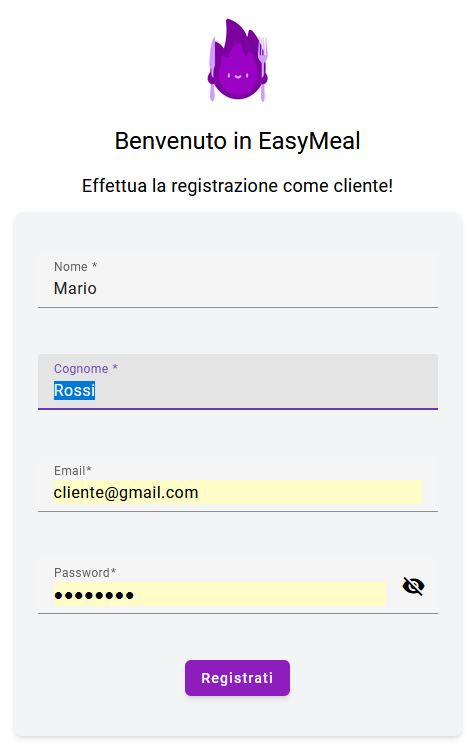
\includegraphics[width=0.9\textwidth]{./img/registrazioneCliente.jpg}
    \caption{Pagina di registrazione del cliente}
    \label{fig:esempio}
\end{figure}

Dopo aver compilato i campi, cliccando il pulsante "Registrati", gli utenti verranno reindirizzati alla propria pagina \textit{home} di pertinenza.



\subsection{Ristoratore} % --------------------- SECTION DEL RISTORATORE ---------------------%

\subsubsection{Accesso ristoratore}
Questa è la schermata di accesso per il ristoratore, dove gli utenti non autenticati possono inserire le proprie credenziali di accesso, costituite dall'\textit{email} e dalla {password}. 
Dopo aver compilato i campi, cliccando il pulsante "Accedi", gli utenti verranno reindirizzati alla propria pagina \textit{home} di pertinenza.

\newpage
\begin{figure}[h]
    \centering
    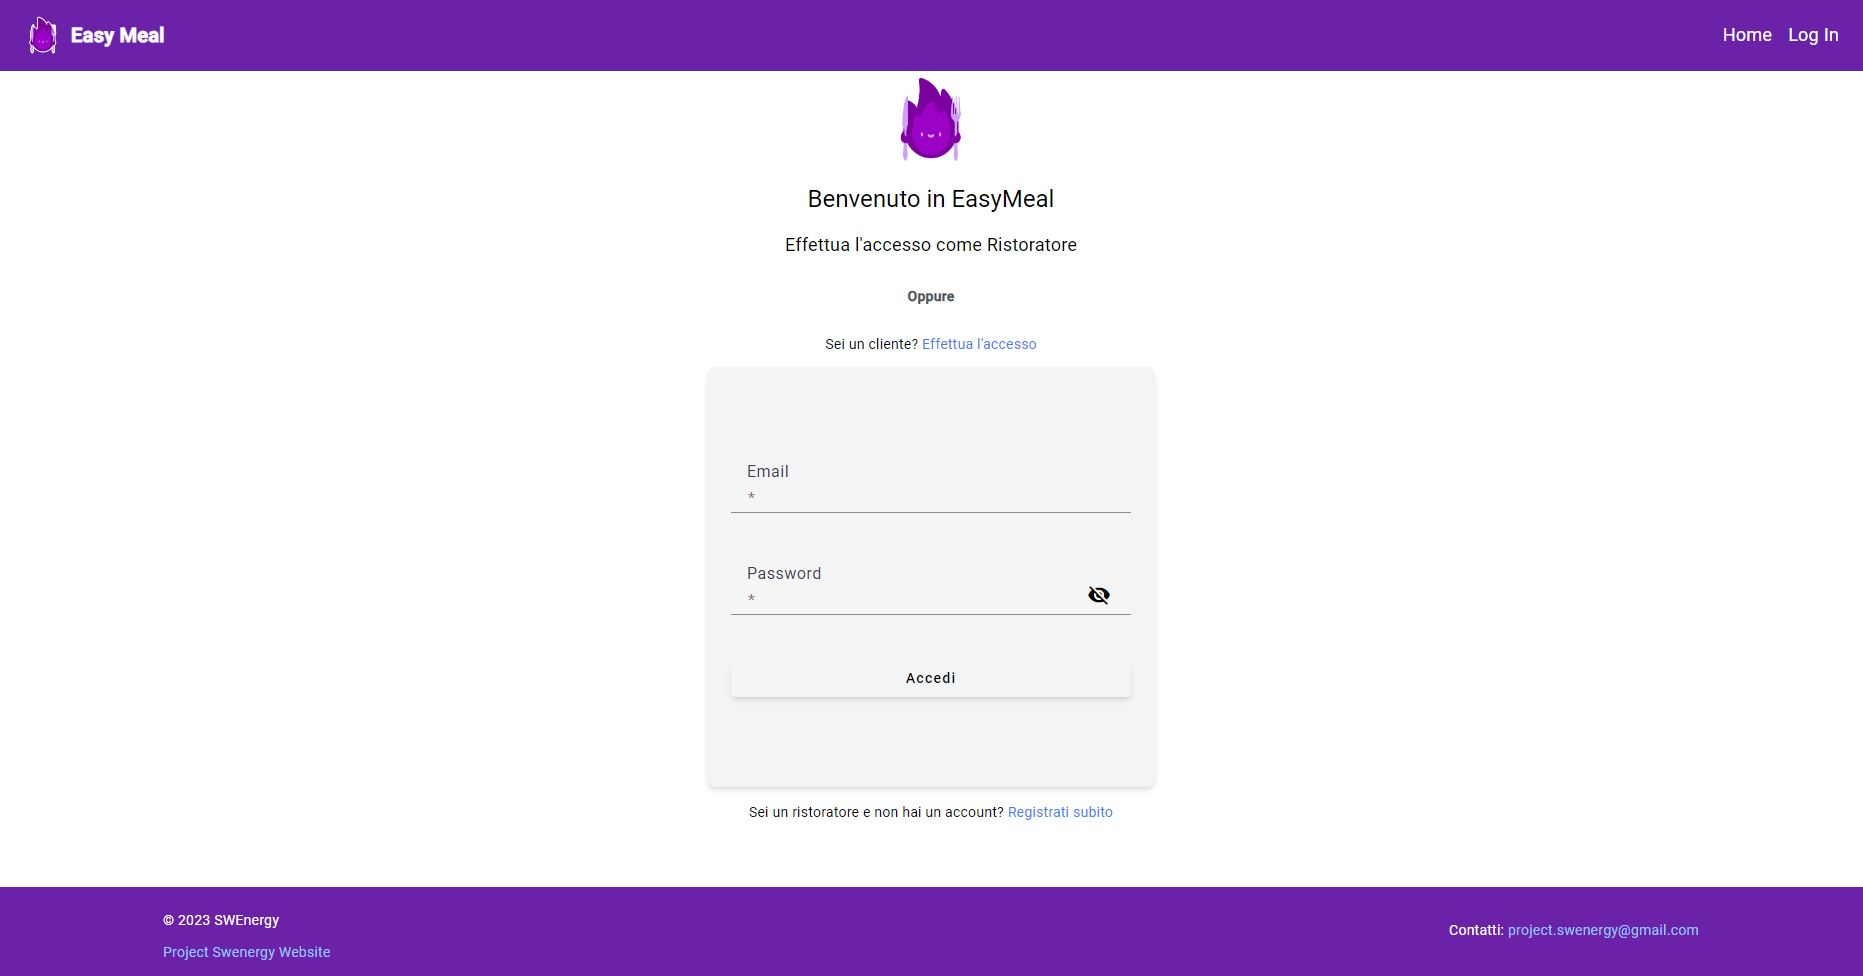
\includegraphics[width=0.9\textwidth]{./img/loginRistoratore.jpg}
    \caption{Pagina di login del ristoratore}
    \label{fig:esempio}
\end{figure}

Qui l'utente, nel caso non fosse registrato, può cliccare sul \textit{link} "Registrati subito" per essere reindirizzato alla pagina di registrazione del ristoratore.
Nel caso l'utente che stia visitando questa pagina non sia un ristoratore, bensì un cliente, può cliccare sul \textit{link} "Sei un cliente? Effettua l'accesso" 
per essere reindirizzato alla pagina di accesso del cliente.

\subsubsection{Permessi non corretti}
Se l'utente non fosse autenticato ad accedere ad una determina pagina, verrò reindirizzato alla seguente schermata:
IMMAGINE DA INSERIRE

\subsubsection{Pagina inesistente}
SE SI FA NEL MVP ALLORA VA MESSA + IMMAGINE, ALTRIMENTI SI CANCELLA QUELLO SCRITTO:
Si noti che se l'utente cerca di accedere ad una pagina che non esiste, verrà reindirizzato alla
seguente schermata, da cui in ogni momento potrà ritornare alla propria pagina principale.

\subsubsection{Registrazione ristoratore}
Questa è la schermata di registrazione per il ristoratore, dove gli utenti che non hanno un \textit{account} possono crearne uno.
Le informazioni da inserire per poter creare un profilo sono le seguenti:
\begin{itemize}
    \item Nome
    \item Cognome
    \item Email
    \item Password
    \item CONTINUARE AD AGGIUNGER IN CASO
\end{itemize}

\begin{figure}[h]
    \centering
    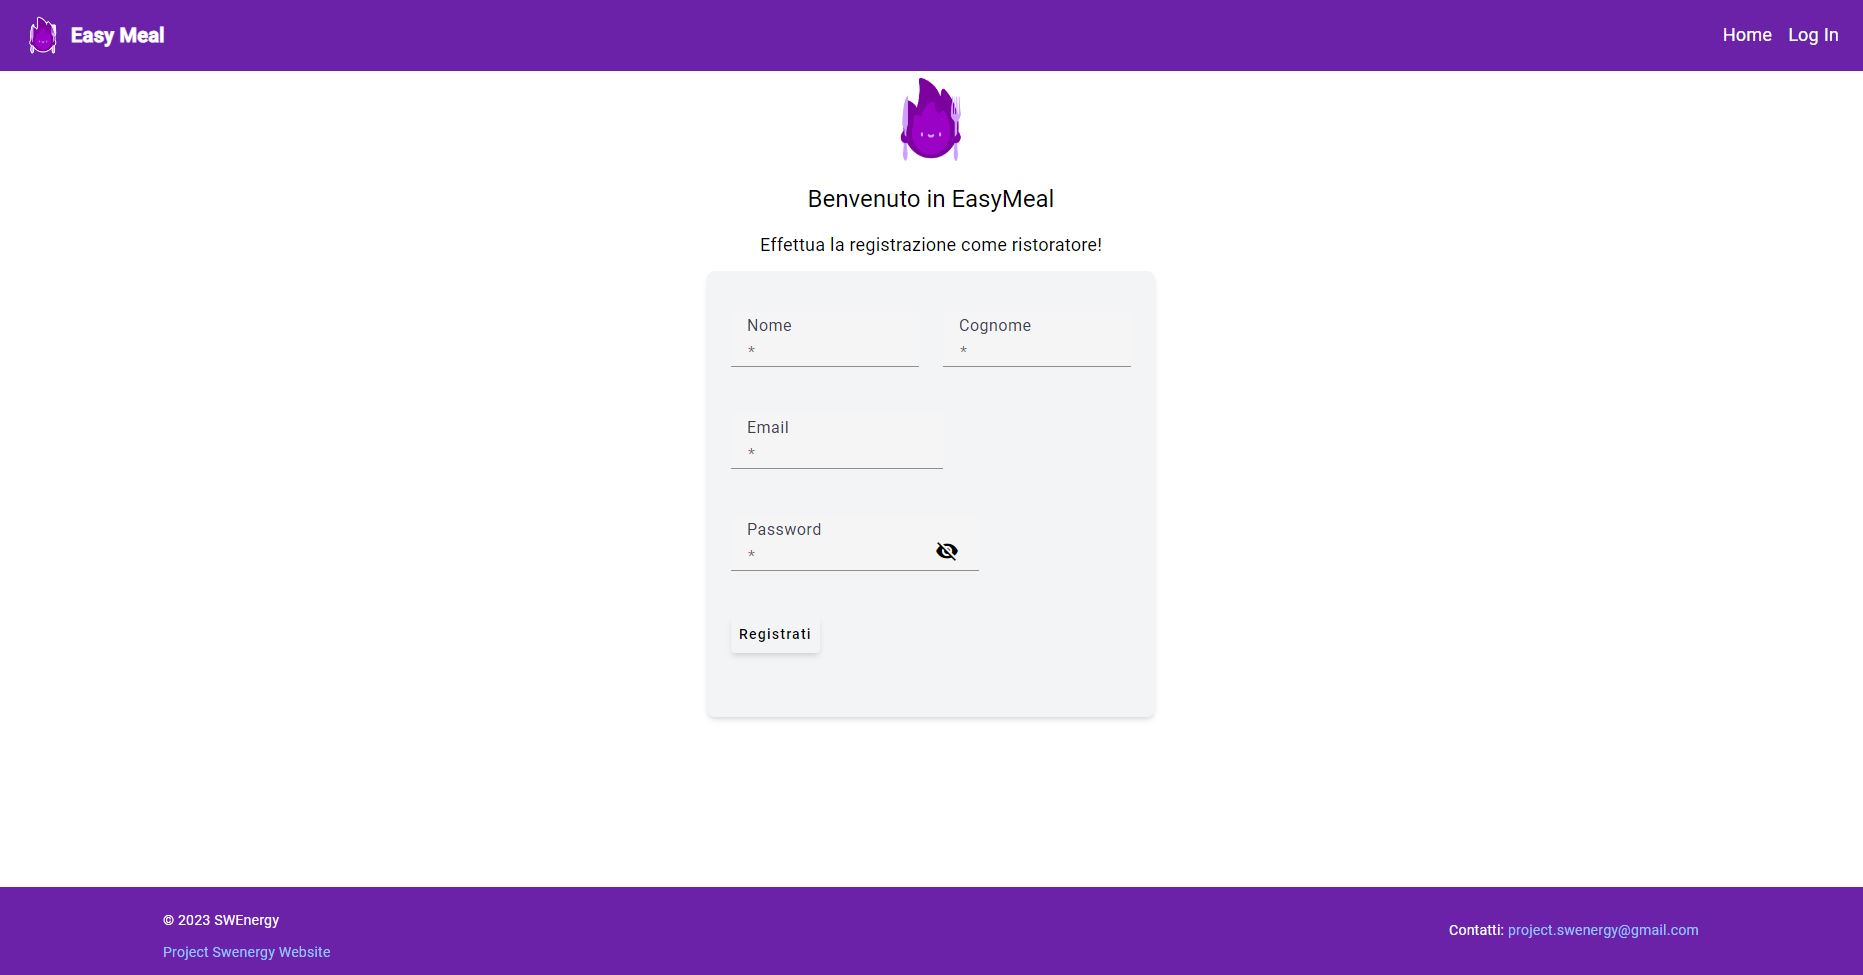
\includegraphics[width=0.9\textwidth]{./img/registrazioneRistoratore.jpg}
    \caption{Pagina di registrazione del ristoratore}
    \label{fig:esempio}
\end{figure}

Dopo aver compilato i campi, cliccando il pulsante "Registrati", gli utenti verranno reindirizzati alla propria pagina \textit{home} di pertinenza.

\section{Supporto tecnico}
Per ogni problema riguardante l'installazione, l'utilizzo o il funzionamento non corretto del \textit{software}, è possibile contattare SWEnergy tramite 
l'indirizzo \textit{email} \href{mailto:project.swenergy@gmail.com}{project.swenergy@gmail.com}, indicato anche nel frontespizio di questo documento. 
Al fine di agevolare la localizzazione dell'\textit{email} nella casella di posta, si raccomanda di scrivere l'oggetto nel seguente formato:
\begin{itemize}
    \item \textbf{Oggetto:} [EasyMeal] - [Nome del problema]
    \item \textbf{Corpo:} 
    \begin{itemize}
        \item Data in cui si è riscontrato il malfunzionamento;
        \item Descrizione dettagliata del problema riscontrato;
        \item Sistema operativo e \textit{browser} in cui si è verificato il problema.
    \end{itemize}
\end{itemize}

Se utile a una miglior comprensione del problema è possibile allegare eventuali \textit{screenshot} o video che mostrino il problema riscontrato. 
Al fine di garantire un supporto tecnico ottimale, ogni \textit{email} inviata verrà automaticamente inoltrata a tutti i membri del gruppo, assicurando così una 
maggiore sicurezza della sua lettura.

\end{document}
